%----------------------------------------------------------------------------------------
%	PACKAGES AND THEMES
%----------------------------------------------------------------------------------------
\documentclass[aspectratio=169,xcolor=dvipsnames]{beamer}
\usetheme{SimplePlus}

\usepackage{amsmath,amssymb,amsfonts,amsthm}
\usepackage{bbm}
\usepackage{mathtools}
\usepackage{xspace}
\usepackage{dsfont}
\usepackage{pifont}
\usepackage{hyperref}
\usepackage{graphicx} % Allows including images
\usepackage{booktabs} % Allows the use of \toprule, \midrule and \bottomrule in tables
\usepackage{fontawesome}
\usepackage{multicol}
\usepackage[
	backend=biber, 
	style=alphabetic, 
	natbib=true, 
	backref=True,
	hyperref=true,
	url=false,
	isbn=false,
	maxcitenames=1,
	maxbibnames=100,
	giveninits=true,
]{biblatex}
\preto\fullcite{\AtNextCite{\defcounter{maxnames}{99}}}
\def\XS{\xspace}
\DeclareMathAlphabet{\mathb}{OML}{cmm}{b}{it}
\def\sbm#1{\ensuremath{\mathb{#1}}}

%% Bold fonts
\def\Ab{{\sbm{A}}\XS}  \def\ab{{\sbm{a}}\XS}
\def\Bb{{\sbm{B}}\XS}  \def\bb{{\sbm{b}}\XS}
\def\Cb{{\sbm{C}}\XS}  \def\cb{{\sbm{c}}\XS}
\def\Db{{\sbm{D}}\XS}  \def\db{{\sbm{d}}\XS}
\def\Eb{{\sbm{E}}\XS}  \def\eb{{\sbm{e}}\XS}
\def\Fb{{\sbm{F}}\XS}  \def\fb{{\sbm{f}}\XS}
\def\Gb{{\sbm{G}}\XS}  \def\gb{{\sbm{g}}\XS}
\def\Hb{{\sbm{H}}\XS}  \def\hb{{\sbm{h}}\XS}
\def\Ib{{\sbm{I}}\XS}  \def\ib{{\sbm{i}}\XS}
\def\Jb{{\sbm{J}}\XS}  \def\jb{{\sbm{j}}\XS}
\def\Kb{{\sbm{K}}\XS}  \def\kb{{\sbm{k}}\XS}
\def\Lb{{\sbm{L}}\XS}  \def\lb{{\sbm{l}}\XS}
\def\Mb{{\sbm{M}}\XS}  \def\mb{{\sbm{m}}\XS}
\def\Nb{{\sbm{N}}\XS}  \def\nb{{\sbm{n}}\XS}
\def\Ob{{\sbm{O}}\XS}  \def\ob{{\sbm{o}}\XS}
\def\Pb{{\sbm{P}}\XS}  \def\pb{{\sbm{p}}\XS}
\def\Qb{{\sbm{Q}}\XS}  \def\qb{{\sbm{q}}\XS}
\def\Rb{{\sbm{R}}\XS}  \def\rb{{\sbm{r}}\XS}
\def\Sb{{\sbm{S}}\XS}  \def\sb{{\sbm{s}}\XS}
\def\Tb{{\sbm{T}}\XS}  \def\tb{{\sbm{t}}\XS}
\def\Ub{{\sbm{U}}\XS}  \def\ub{{\sbm{u}}\XS}
\def\Vb{{\sbm{V}}\XS}  \def\vb{{\sbm{v}}\XS}
\def\Wb{{\sbm{W}}\XS}  \def\wb{{\sbm{w}}\XS}
\def\Xb{{\sbm{X}}\XS}  \def\xb{{\sbm{x}}\XS}
\def\Yb{{\sbm{Y}}\XS}  \def\yb{{\sbm{y}}\XS}
\def\Zb{{\sbm{Z}}\XS}  \def\zb{{\sbm{z}}\XS}

\def\alphab      {{\sbmm{\alpha}}\XS}
\def\betab       {{\sbmm{\beta}}\XS}
\def\gammab      {{\sbmm{\gamma}}\XS}      \def\Gammab    {{\sbmm{\Gamma}}\XS}
\def\deltab      {{\sbmm{\delta}}\XS}      \def\Deltab    {{\sbmm{\Delta}}\XS}
\def\epsilonb    {{\sbmm{\epsilon}}\XS}
\def\varepsilonb {{\sbmm{\varepsilon}}\XS}
\def\etab        {{\sbmm{\eta}}\XS}
\def\thetab      {{\sbmm{\theta}}\XS}      \def\Thetab    {{\sbmm{\Theta}}\XS}
\def\varthetab   {{\sbmm{\vartheta}}\XS}
\def\iotab       {{\sbmm{\iota}}\XS}
\def\kappab      {{\sbmm{\kappa}}\XS}
\def\lambdab     {{\sbmm{\lambda}}\XS}    \def\Lambdab   {{\sbmm{\Lambda}}\XS}
\def\mub         {{\sbmm{\mu}}\XS}
\def\nub         {{\sbmm{\nu}}\XS}
\def\xib         {{\sbmm{\xi}}\XS}                 \def\Xib        {{\sbmm{\Xi}}\XS}
\def\pib         {{\sbmm{\pi}}\XS}                 \def\Pib        {{\sbmm{\Pi}}\XS}
\def\varpib      {{\sbmm{\varpi}}\XS}
\def\rhob        {{\sbmm{\rho}}\XS}
\def\varrhob     {{\sbmm{\varrho}}\XS}
\def\sigmab      {{\sbmm{\sigma}}\XS}      \def\Sigmab    {{\sbmm{\Sigma}}\XS}
\def\varsigmab   {{\sbmm{\varsigma}}\XS}  \def\Varsigmab {{\sbmm{\Varsigma}}\XS}
\def\phib        {{\sbmm{\phi}}\XS}        \def\Phib       {{\sbmm{\Phi}}\XS}
\def\varphib     {{\sbmm{\varphi}}\XS}
\def\chib        {{\sbmm{\chi}}\XS}
\def\psib        {{\sbmm{\psi}}\XS}        \def\Psib       {{\sbmm{\Psi}}\XS}
\def\omegab      {{\sbmm{\omega}}\XS}      \def\Omegab    {{\sbmm{\Omega}}\XS}
\def\taub        {{\sbmm{\tau}}\XS}
\def\upsilonb    {{\sbmm{\upsilon}}\XS}   \def\Upsilonb  {{\sbmm{\Upsilon}}\XS}
\def\zetab       {{\sbmm{\zeta}}\XS}

\def\pth#1{\left(#1\right)}                \def\bigpth#1{\bigl(#1\bigr)}              \def\I{\,|\,}           % "sachant" bien espac\'e pour 

\def\Abb{{\sbl{A}}\XS}  \def\abb{{\sbl{a}}\XS}
\def\Bbb{{\sbl{B}}\XS}  \def\bbb{{\sbl{b}}\XS}
\def\Cbb{{\sbl{C}}\XS}  \def\cbb{{\sbl{c}}\XS}
\def\Dbb{{\sbl{D}}\XS}  \def\dbb{{\sbl{d}}\XS}
\def\Ebb{{\sbl{E}}\XS}  \def\ebb{{\sbl{e}}\XS}
\def\Fbb{{\sbl{F}}\XS}  \def\fbb{{\sbl{f}}\XS}
\def\Gbb{{\sbl{G}}\XS}  \def\gbb{{\sbl{g}}\XS}
\def\Hbb{{\sbl{H}}\XS}  \def\hbb{{\sbl{h}}\XS}
\def\Ibb{{\sbl{I}}\XS}  \def\ibb{{\sbl{i}}\XS}
\def\Jbb{{\sbl{J}}\XS}  \def\jbb{{\sbl{j}}\XS}
\def\Kbb{{\sbl{K}}\XS}  \def\kbb{{\sbl{k}}\XS}
\def\Lbb{{\sbl{L}}\XS}  \def\lbb{{\sbl{l}}\XS}
\def\Mbb{{\sbl{M}}\XS}  \def\mbb{{\sbl{m}}\XS}
\def\Nbb{{\sbl{N}}\XS}  \def\nbb{{\sbl{n}}\XS}
\def\Obb{{\sbl{O}}\XS}  \def\obb{{\sbl{o}}\XS}
\def\Pbb{{\sbl{P}}\XS}  \def\pbb{{\sbl{p}}\XS}
\def\Qbb{{\sbl{Q}}\XS}  \def\qbb{{\sbl{q}}\XS}
\def\Rbb{{\sbl{R}}\XS}  \def\rbb{{\sbl{r}}\XS}
\def\Sbb{{\sbl{S}}\XS}  \def\sbb{{\sbl{s}}\XS}
\def\Tbb{{\sbl{T}}\XS}  \def\tbb{{\sbl{t}}\XS}
\def\Ubb{{\sbl{U}}\XS}  \def\ubb{{\sbl{u}}\XS}
\def\Vbb{{\sbl{V}}\XS}  \def\vbb{{\sbl{v}}\XS}
\def\Wbb{{\sbl{W}}\XS}  \def\wbb{{\sbl{w}}\XS}
\def\Xbb{{\sbl{X}}\XS}  \def\xbb{{\sbl{x}}\XS}
\def\Ybb{{\sbl{Y}}\XS}  \def\ybb{{\sbl{y}}\XS}
\def\Zbb{{\sbl{Z}}\XS}  \def\zbb{{\sbl{z}}\XS}
% TEX 7(ascii) bits
%
% ABRMATH.tex           LaTeX document
% Author: PC          Date  : Juillet 1996
% Raccourcis d'expressions tres usitees en math
% Derniere modif importante le 12-08-2000 pour ma th�e

\def\prox#1{\mathrm{prox}_{#1}}
\newcommand{\vertiii}[1]{{\left\vert\kern-0.25ex\left\vert\kern-0.25ex\left\vert #1 
		\right\vert\kern-0.25ex\right\vert\kern-0.25ex\right\vert}}

%-- Accolades, parenth�es, etc --------------------------------------
        
\def\pth#1{\left(#1\right)}                \def\stdpth#1{(#1)}
\def\acc#1{\left\{#1\right\}}              \def\stdacc#1{\{#1\}}
\def\cro#1{\left[#1\right]}                \def\stdcro#1{[#1]}
\def\bars#1{\left|#1\right|}               \def\stdbars#1{|#1|}
\def\norm#1{\left\|#1\right\|}             \def\stdnorm#1{\|#1\|}
\def\scal#1{\left\langle#1\right\rangle}   \def\stdscal#1{\langle#1\rangle}
 
\def\bigpth#1{\bigl(#1\bigr)}              \def\biggpth#1{\biggl(#1\biggr)}
\def\bigacc#1{\bigl\{#1\bigr\}}            \def\biggacc#1{\biggl\{#1\biggr\}}
\def\bigcro#1{\bigl[#1\bigr]}              \def\biggcro#1{\biggl[#1\biggr]}
\def\bigbars#1{\bigl|#1\bigr|}             \def\biggbars#1{\biggl|#1\biggr|}
\def\bignorm#1{\bigl\|#1\bigr\|}           \def\biggnorm#1{\biggl\|#1\biggr\|}
\def\bigscal#1{\bigl\langle#1\bigr\rangle} \def\biggscal#1{\biggl\langle#1\biggr\rangle}

\def\Bigpth#1{\Bigl(#1\Bigr)}              \def\Biggpth#1{\Biggl(#1\Biggr)}
\def\Bigacc#1{\Bigl\{#1\Bigr\}}            \def\Biggacc#1{\Biggl\{#1\Biggr\}}
\def\Bigcro#1{\Bigl[#1\Bigr]}              \def\Biggcro#1{\Biggl[#1\Biggr]}
\def\Bigbars#1{\Bigl|#1\Bigr|}             \def\Biggbars#1{\Biggl|#1\Biggr|}
\def\Bignorm#1{\Bigl\|#1\Bigr\|}           \def\Biggnorm#1{\Biggl\|#1\Biggr\|}
\def\Bigscal#1{\Bigl\langle#1\Bigr\rangle} \def\Biggscal#1{\Biggl\langle#1\Biggr\rangle}


% Quelques fonctions classiques + Arguments entre [] ----------------
%
% Laisser les \mathrm entre {}, sinon � d�onne dans le style "ieeetran". 
%
\def\diag{{\mathrm{diag}}}		\def\Diag#1{{\mathrm{diag}}\bigcro{#1}}	\def\Diagold#1{{\mathrm{diag}}\cro{#1}}
\def\tr{{\mathrm{tr}}\,}		\def\Tr#1{{\mathrm{tr}}\bigcro{#1}}			\def\Trold#1{{\mathrm{tr}}\cro{#1}}
\def\rg{{\mathrm{rg}}\,}		\def\Rg#1{{\mathrm{rg}}\bigcro{#1}}			\def\Rgold#1{{\mathrm{rg}}\cro{#1}}
\def\esp{{\mathrm{E}}\,}		\def\Esp#1{{\mathrm{E}}\bigcro{#1}}					\def\Espud#1#2{{\mathrm{E}}_{#1}\bigcro{#2}}			\def\Espold#1{{\mathrm{E}}\cro{#1}} 
\def\var{{\mathrm{var}}\,}		\def\Var#1{{\mathrm{var}}\bigcro{#1}}		\def\Varold#1{{\mathrm{var}}\cro{#1}}
\def\cov{{\mathrm{Cov}}\,}		\def\Cov#1{{\mathrm{Cov}}\bigcro{#1}}		\def\Covold#1{{\mathrm{Cov}}\cro{#1}}
\def\Cos#1{\cos\bigcro{#1}}	\def\Cosold#1{\cos\cro{#1}}
\def\Sin#1{\sin\cro{#1}}		\def\Sinold#1{\sin\cro{#1}}
\def\Exp#1{\exp\bigcro{#1}}	\def\Expold#1{\exp\cro{#1}}
\def\Log#1{\log\bigcro{#1}}	\def\Logold#1{\log\cro{#1}}
\def\Ln#1{\ln\cro{#1}}			\def\Det#1{\det\bigcro{#1}}					\def\Detold#1{\det\cro{#1}}

\def\cond{\textrm{Cond}\,}		\def\Cond#1{\cond\bigpth{#1}}

\def\sinc{{\mathrm{sinc}}\,}	\def\Sinc#1{{\mathrm{sinc}}\bigcro{#1}}	\def\Sincold#1{{\mathrm{sinc}}\cro{#1}}
\def\rang{{\mathrm{rang}}\,}	\def\Rang#1{\rang\bigcro{#1}}					\def\Rangold#1{\rang\cro{#1}}
\def\ker{\textrm{Ker}\,}		\def\Ker#1{\ker\bigcro{#1}}					\def\Kerold#1{\ker\cro{#1}}
\def\img{\textrm{Im}\,}			\def\Img#1{\img\bigcro{#1}}					\def\Imgold#1{\img\cro{#1}}
\def\vect{{\mathrm{Vect}}\,}	\def\Vect#1{\vect\bigcro{#1}}					\def\Vectold#1{\vect\cro{#1}}
\def\sgn{{\mathrm{sgn}}}		\def\Sgn#1{\sgn\bigcro{#1}}					\def\Sgnold#1{\sgn\cro{#1}}

% Signe proba
\def\Pr{\mathop{\textrm{Pr}}}

% Variante pour \Re:
\def\reel{{\mathrm{Re}}} 		\def\Reel#1{{\mathrm{Re}}\cro{#1}}
\def\card{{\mathrm{Card}}}		\def\Card#1{{\mathrm{Card}}\cro{#1}}

\def\sh{{\mathrm{sh}}}                % sin hyperbolique en FR
\def\ch{{\mathrm{ch}}}                % cos hyperbolique en FR
\def\th{{\mathrm{th}}}                % th hyperbolique en FR
\def\coth{{\mathrm{coth}}}            % cot hyperbolique en FR
\def\div{{\mathrm{div}}}              % divergence
\def\rotv{\overrightarrow{\mathop{{\mathrm{rot}}}}}    % rotationnel avec fleche
\def\gradv{\overrightarrow{\mathop{{\mathrm{grad}}}}}  % gradient avec fleche
\def\coeffbin#1#2{\pth{\setlength{\arraycolsep}{.1em}\barr{c}#1\\#2\earr}}
% Remarque : \exist \binom{}{}

%-- Textes (if, si,...) droit en math ---------------------------

\def\IF{\text{if\:}}            % \def\SI{\text{si\:}}
\def\If{\text{If\:}}             \def\Si{\text{Si\:}}
\def\AND{\text{and\:}}           \def\ET{\text{et\:}}
\def\OR{\text{or\:}}             \def\OU{\text{ou\:}}
\def\THEN{\text{then\:}}         \def\ALORS{\text{alors\:}}
                                 \def\DOU{\text{d'o\`u\:}}
\def\WHERE{\text{where\:}}       \def\Ou{\text{o\`u\:}}
\def\WHEN{\text{when\:}}         \def\QUAND{\text{quand\:}}
\def\FOR{\text{for\:}}           \def\POUR{\text{pour\:}}
\def\FORALL{\text{for all\:}}    \def\POURTOUT{\text{pour tout\:}}
\def\ST{\text{s.t.\:}}           \def\SC{\text{s.c.\:}}
\def\SUBJTO{\text{subject to\:}} \def\SOUSC{\text{sous contraintes\:}}
\def\OTHERWISE{\text{otherwise}} \def\SINON{\text{sinon}}
\def\WITH{\text{with\:}}         \def\AVEC{\text{avec\:}}
\def\IN{\text{in\:}}             \def\DANS{\text{dans\:}}

%-- Triture param�res tableaux... -----------------------------

\def\arrayp{\renewcommand{\arraystretch}{.7}\setlength{\arraycolsep}{2pt}}
\def\tabp{\renewcommand{\arraystretch}{.7}\setlength{\tabcolsep}{2pt}}

%-- Environnement encadr\'e ------------------------------------
% Ces d\'efinitons introduisent un nouvel environnement appele "fminipage". Il 
% permet d'encadrer une partie de texte.

\newsavebox{\fminibox}
\newlength{\fminilength}
\newenvironment{fminipage}[1][\linewidth]
  {\setlength{\fminilength}{#1}%-2\fboxsep-2\fboxrule}%
   \begin{lrbox}{\fminibox}\begin{minipage}{\fminilength}}
  {\end{minipage}\end{lrbox}\noindent\fbox{\usebox{\fminibox}}}

%-- Divers : "^{-1}", "dag", "," ... %---------------------------

\def\M{^{-1}} 
\def\T{^\tD} 
\def\+{^\dagger}
\def\I{\,|\,}           % "sachant" bien espac\'e pour les formules
\def\J{\mathop{\,;\,}}  % "point virgule" bien espac\'e pour les formules.
\def\w{,\thinspace}
\def\W{,\thickspace}
\def\ldotsv{,\,\ldots,\,}
\def\V{,}               % Virgule pour les nombres decimaux
%\def\V{.}              % Point pour les anglo-saxons
\def\e#1{.10^{#1}}      % Notation scientifique a la francaise
%\def\e#1{\rm{e}^{#1}}  % Notation scientifique anglo-saxonne

\def\egdef{\stackrel{\Delta}{=}}
\def\nequiv{\not\kern-.05em\equiv}
\def\egal{\kern-.5em=\kern-.5em}        % Moins d'espace autour de "="
\def\propt{\kern-.2em\propto\kern-.2em} % Idem
\def\dans{\in\!}                        % Trop d'espace apres "appartient a"
\def\pourtt{\forall\,}                  % Pas assez d'espace
\def\wh#1{\widehat{#1}}                 % Sombrero !
\def\wt#1{\widetilde{#1}} 

%\def\arg{\mathop{\mathrm{arg}}}
\def\argmax{\mathop{\mathrm{arg\,max}}} % Mieux que \def\argmax{\arg\max}
\def\argmin{\mathop{\mathrm{arg\,min}}} % car l'indice est reparti
\def\EL{\mathrm{EL}}
\def\Vect{\mathop{\text{Vect}}}

\def\froc#1#2{{#1/#2}}                  % Frac en toc
\def\fric#1#2{\frac1{#2}#1}
\def\fracds#1#2{\frac{\displaystyle#1}{\displaystyle#2}}
\def\diff#1#2{{\frac{\mathop{}\!\mathrm{d}#1}{\mathop{}\!\mathrm{d}#2}}}
\def\doff#1#2{{\froc{\mathop{}\!\mathrm{d}#1}{\mathop{}\!\mathrm{d}#2}}}
\def\dif{\mathop{}\!\mathrm{d}}

\def\dd{\,d}                            % doit etre en italique en anglais
%\def\dd{\,\dD}                         % doit etre droit en francais
\def\derpar#1#2{{\frac{\partial #1}{\partial #2}}}
\def\derpor#1#2{{\froc{\partial #1}{\partial #2}}}
\def\parsec#1#2#3{{\frac{\partial^2 #1}{\partial #2\,\partial #3}}}
\def\parsecd#1#2{{\frac{\partial^2 #1}{{\partial #2}^2}}}
\def\porsec#1#2#3{{\froc{\partial^2 #1}{\partial #2\,\partial #3}}}
\def\porsecd#1#2{{\froc{\partial^2 #1}{{\partial #2}^2}}}
\def\derpark#1#2#3{{\frac{\partial^{#3} #1}{\partial #2^{#3}}}}

\def\intdouble{\int\kern-0.3em\int}
\def\inttriple{\int\kern-0.3em\int\kern-0.3em\int}
\def\prods{\mathop{\text{\footnotesize$\displaystyle\prod$}}}

% Pour mettre un \No{} au-dessus d'une lettre (\TM, 02/97) (package{amsmath.sty})
\def\rond#1{\overset{\kern-0.33em~_\circ}{#1}}
\def\rondit[#1]#2{\overset{\kern#1~_\circ}{#2}}

% Pour mettre un texte dans un rond : (utilise pstricks ; \JI, 08/97)
\def\incirc#1{\pscirclebox[framesep=1pt]{\scriptsize#1}}
\def\incircp#1{\pscirclebox[framesep=1pt]{\tiny#1}}
\def\outcirc#1{\raisebox{-3pt}{\huge$\times$}\hspace*{-.45cm}\text{\incirc{#1}}}


%%%%%%%% def Fourier %%%%%%%%%%%%%%%%%%%
\def\sss{\scriptscriptstyle}
\def\idft{\textsc{idft}}
\def\tfd{{\sc tfd}\XS}
\def\fft{{\sf fft}\xspace}
\def\ifft{{\sf ifft}\xspace}
\def\fric#1#2{#1\text{{\Large /}}#2} % Frac en toc 	  
\def\Wfou{W_{\sss NP}\XS}
\def\FFou{W_{\sss PP}\+\XS}
\def\FFoud{W_{\sss PP}\XS}
\def\WcFou{\Wc_{\sss N}\XS}

\usepackage[dvipsnames]{xcolor}
\usepackage{tikz}
\usetikzlibrary{backgrounds}
\usetikzlibrary{arrows,shapes}
\usetikzlibrary{tikzmark}
\usetikzlibrary{calc}

\usepackage{mathtools, nccmath}
\usepackage{wrapfig}
\usepackage{comment}



% table alignment
\usepackage{array}
\usepackage{ragged2e}
\newcolumntype{P}[1]{>{\RaggedRight\hspace{0pt}}p{#1}}
\newcolumntype{X}[1]{>{\RaggedRight\hspace*{0pt}}p{#1}}

% color box
\usepackage{tcolorbox}


% for tikz
\usepackage{tikz}
%\usetikzlibrary{trees}
\usetikzlibrary{arrows,shapes,positioning,shadows,trees,mindmap}
% \usepackage{forest}
\usepackage[edges]{forest}
\usetikzlibrary{arrows.meta}
\colorlet{linecol}{black!75}
\usepackage{xkcdcolors} % xkcd colors


% for colorful equation
\usepackage{tikz}
\usetikzlibrary{backgrounds}
\usetikzlibrary{arrows,shapes}
\usetikzlibrary{tikzmark}
\usetikzlibrary{calc}
% Commands for Highlighting text -- non tikz method
\newcommand{\highlight}[2]{\colorbox{#1!17}{$\displaystyle #2$}}
%\newcommand{\highlight}[2]{\colorbox{#1!17}{$#2$}}
\newcommand{\highlightdark}[2]{\colorbox{#1!47}{$\displaystyle #2$}}

% my custom colors for shading
\colorlet{mhpurple}{Plum!80}


% Commands for Highlighting text -- non tikz method
\renewcommand{\highlight}[2]{\colorbox{#1!17}{#2}}
\renewcommand{\highlightdark}[2]{\colorbox{#1!47}{#2}}

% Some math definitions
\newcommand{\lap}{\mathrm{Lap}}
\newcommand{\pr}{\mathrm{Pr}}

\newcommand{\Tset}{\mathcal{T}}
\newcommand{\Dset}{\mathcal{D}}
\newcommand{\Rbound}{\widetilde{\mathcal{R}}}
\usepackage{tikz}
\usetikzlibrary{tikzmark}
%----------------------------------------------------------------------------------------
%	TITLE PAGE
%----------------------------------------------------------------------------------------

\title[Advanced deep neural networks for MRI image reconstruction]{Advanced deep neural networks for MRI image reconstruction from highly undersampled data in challenging acquisition settings
} % The short title appears at the bottom of every slide, the full title is only on the title page
\subtitle{PhD defense}

\author[Zaccharie] {Zaccharie Ramzi}
% XXX: add supervisors
% XXX: add university and ED
\institute[Inria-CEA] % Your institution as it will appear on the bottom of every slide, may be shorthand to save space
{
    Parietal team, Inria Saclay \\
    NeuroSpin and Cosmostat, CEA Saclay
}
\date{18th February 2022} % Date, can be changed to a custom date

\addbibresource{ThesisBib.bib}
\addbibresource{websites.bib}


\setbeamerfont{subsection in toc}{size=\small}
\setbeamerfont{section in toc}{size=\large}
\setbeamertemplate{blocks}[rounded]%
[shadow=true]


% debug
% \makeatletter
% \begingroup
% \edef\get@@version{\def\noexpand\get@version##1\detokenize{TeX Live}##220##3##4##5)##6\noexpand\@nil}
% \get@@version{\gdef\TeXLiveVersion{20#3#4}}
% \expandafter\get@version\pdftexbanner\@nil
% \endgroup
% \makeatother

%----------------------------------------------------------------------------------------
%	PRESENTATION SLIDES
%----------------------------------------------------------------------------------------

\begin{document}

\begin{frame}
    % Print the title page as the first slide
    \titlepage
    % XXX: add logos
\end{frame}

% Introduction: the problem at hand
% Introduction: physics of MRI
% Acceleration: classics
% Acceleration: CS
% Deep Learning
% Application of DL to MRI: model agnostic, single domain and unrolled networks
% Clinical applicability
% Going further !
% CCL
{
\usebackgroundtemplate{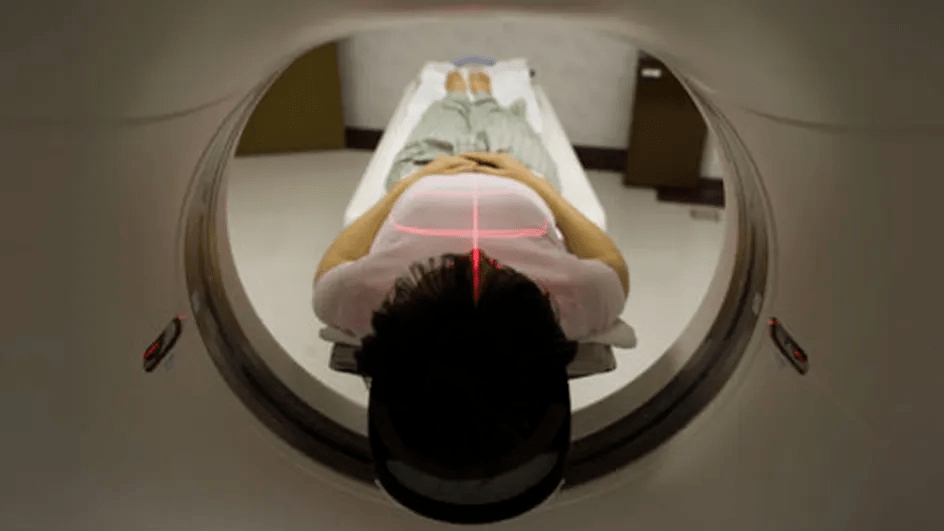
\includegraphics[width=\paperwidth]{Figures/inside_mri.png}}
\begin{frame}[plain]
    % I would like to have the picture of inside the MRI
    % and pass the sound of an MRI scan
    %  \href{run:sons/extract.mp3}{\beamerbutton{écouter}} (https://texnique.fr/osqa/questions/2988/du-son-dans-beamer)
    % https://www.francetvinfo.fr/sante/malgre-l-augmentation-des-besoins-medicaux-le-deficit-en-france-d-appareils-irm-se-fait-de-plus-en-plus-sentir_220301.html
    \href{run:Sounds/mri_sounds.mp3}{\faPlayCircle}
    % XXX: add credit to image
\end{frame}
}

% link between the 2: this is the sound you hear when undergoing an MRI
% now imagine that you will on average hear this during x minutes
% MRI scanners being slow not only generate discomfort but have other impacts on their efficiency...
\begin{frame}{MRI is slow}
    % for debug
    % This has been run with \TeX~Live~\TeXLiveVersion.
    Typical MRI~(Magnetic Resonance Imaging) scan duration: 15 minutes (up to 90 minutes).
    Hence:
    \begin{itemize}
        \item discomfort \& accessibility issues;
        \item reduced patient throughput;
        \item increased motion.
    \end{itemize}
    % give typical duration (compare to CT)
    % give associated problems
    % XXX: add citation for duration
\end{frame}

\begin{frame}{Our objective: accelerate MRI scans}
    % give TOC
    \begin{multicols}{2}
    \tableofcontents
    \end{multicols}
\end{frame}

\section{Introduction to MRI}
\begin{frame}{What does an MRI look like?}
    \begin{figure}
        \centering
        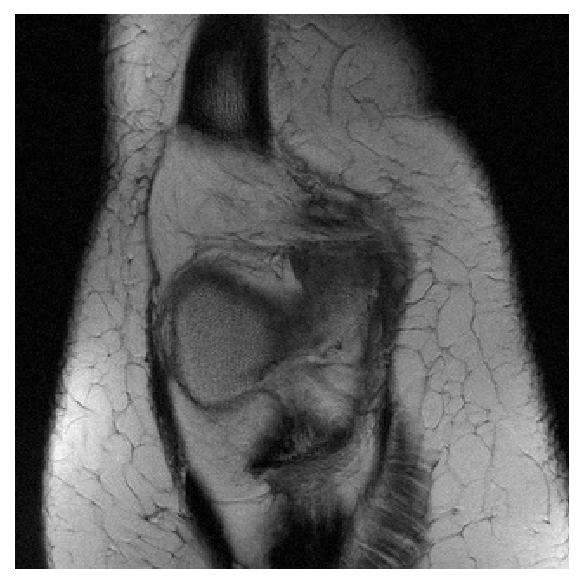
\includegraphics[height=0.6\textheight]{Figures/intro_figures/example_knee_fastmri.pdf}
        \caption{\label{fig:mri-example} \textbf{Example of an MR image}: MR image of the knee taken from the fastMRI dataset.\footfullcite{Zbontar}}
    \end{figure}
\end{frame}

\subsection{Importance of MRI}
\begin{frame}{Importance of MRI - 1}
    % how many MRI scans / scanners
    % how likely is it that you will get an MRI in your life
    Based on a rough extrapolation of the following figure, there is a 99.9\% chance that you will get an MRI in your life in France.
    \begin{figure}
        \centering
        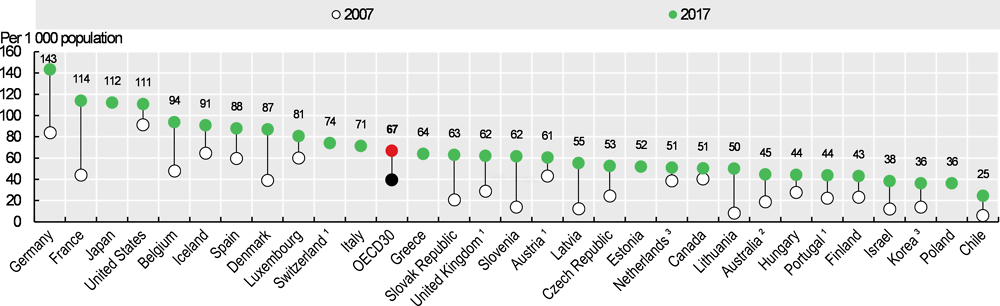
\includegraphics[width=\textwidth]{Figures/intro_figures/num_mri_scans.png}
        \caption{\label{fig:num-mri-scans} \textbf{Number of MRI scans per year per 1000 population}: figure courtesy of \citet{OECDMRI}.}
    \end{figure}
\end{frame}

% There is a reason for that: MRI can help diagnose many different conditions
\begin{frame}{Importance of MRI - 2}
    % list of conditions
    \begin{figure}
        \centering
        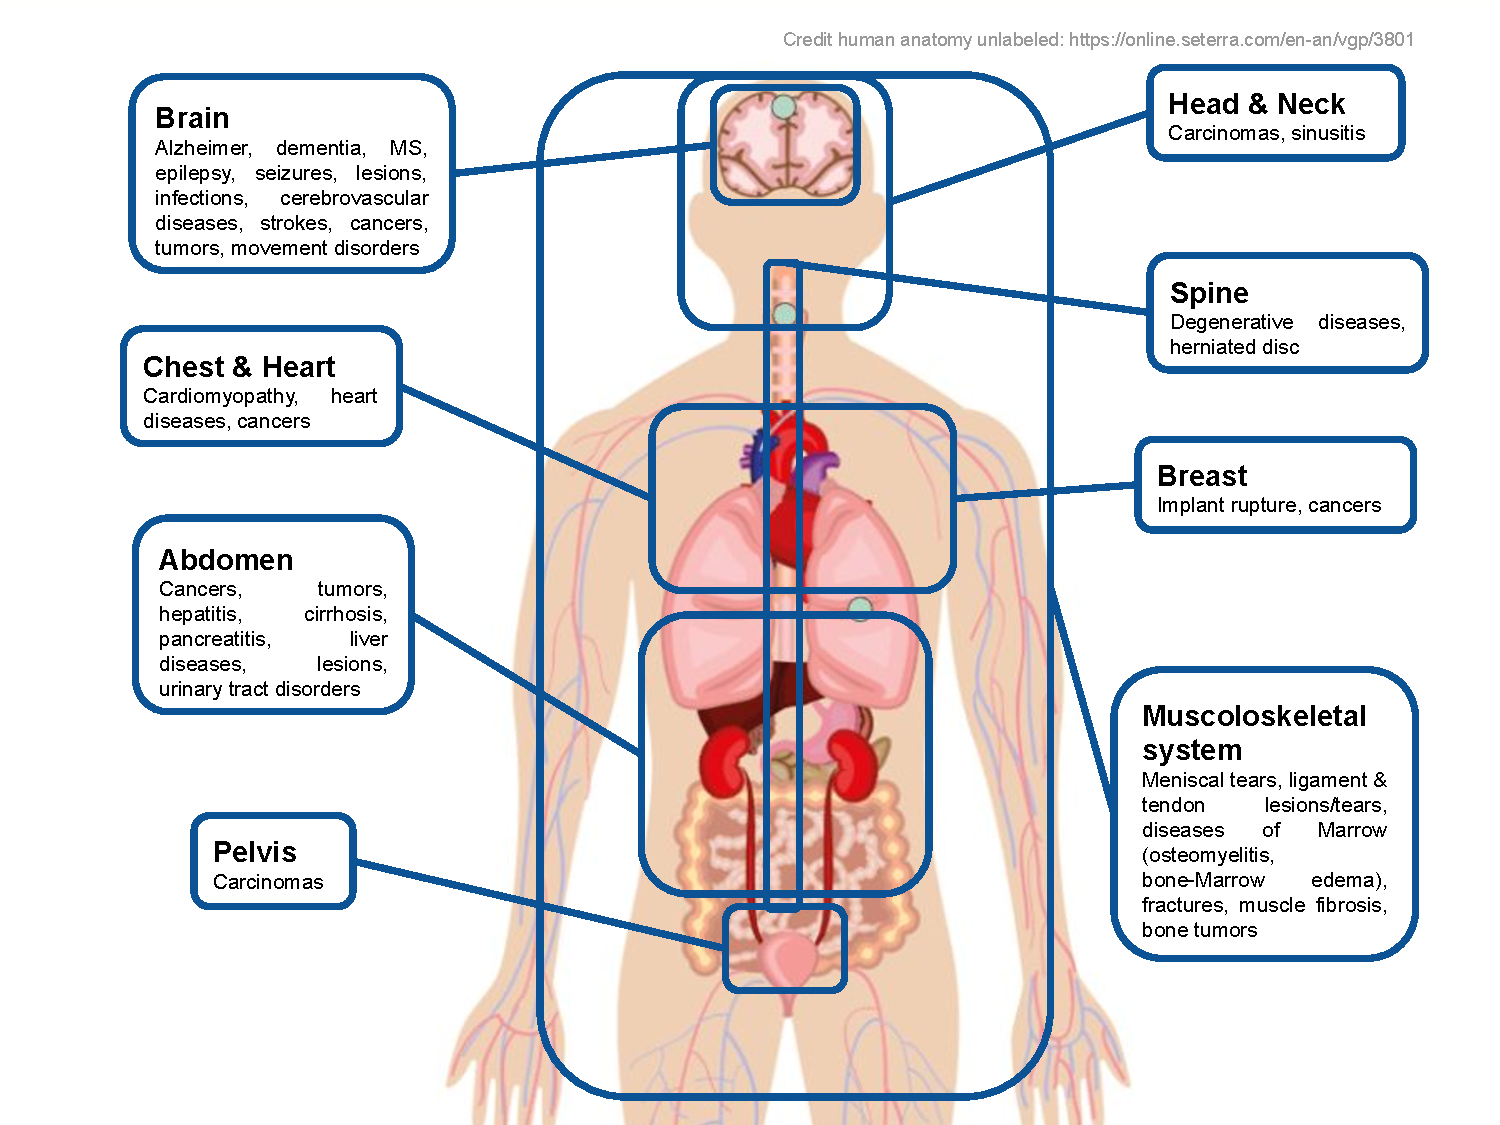
\includegraphics[height=0.6\textheight]{Figures/intro_figures/What_can_we_diagnose_with_MRI.pdf}
        \caption{\label{fig:diagnose-mri} \textbf{What can we diagnose with MRI?} This illustration provides a non-exhaustive list of all the diagnoses that can be carried out with MRI. All the information was compiled from the works of \citet{reimer2010clinical,runge2019essentials}.}
    \end{figure}
\end{frame}

\subsection{Physics of MRI}
% MRI is so popular why isnt it solved already ?
\begin{frame}{Physics of MRI - 1}
    % at its core MRI relies on the MR phenomenon
    % in short: a spin is aligned with the magnetic field, when an RF pulse is sent, it tips the spin in the orthogonal plane before the spin realigns with the magnetic field sending another RF pulse
    \only<1>{
    \begin{figure}
        \centering
        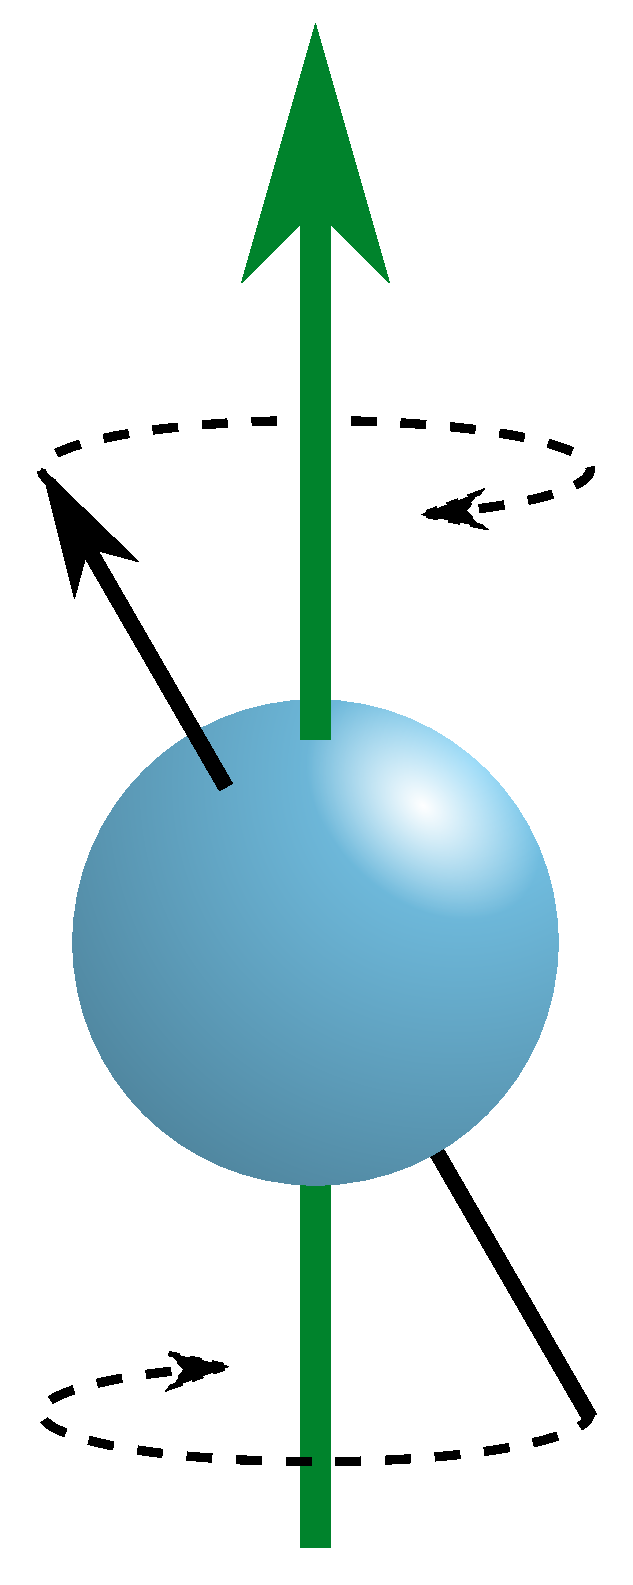
\includegraphics[width=0.14\textwidth]{Figures/intro_figures/Precession_in_magnetic_field.pdf}
        \caption{\label{fig:precession}\textbf{Illustration of the precession of a spin in a magnetic field:} the green arrow represents the $\Bb_0$ magnetic field, while the black arrow represents the magnetic moment of the particle. Illustration courtesy of \citet{wiki}.}
    \end{figure}
    }
    % XXX: add vspace somewhere to avoid the jump effect
    \only<2>{
    \begin{figure}
        \centering
        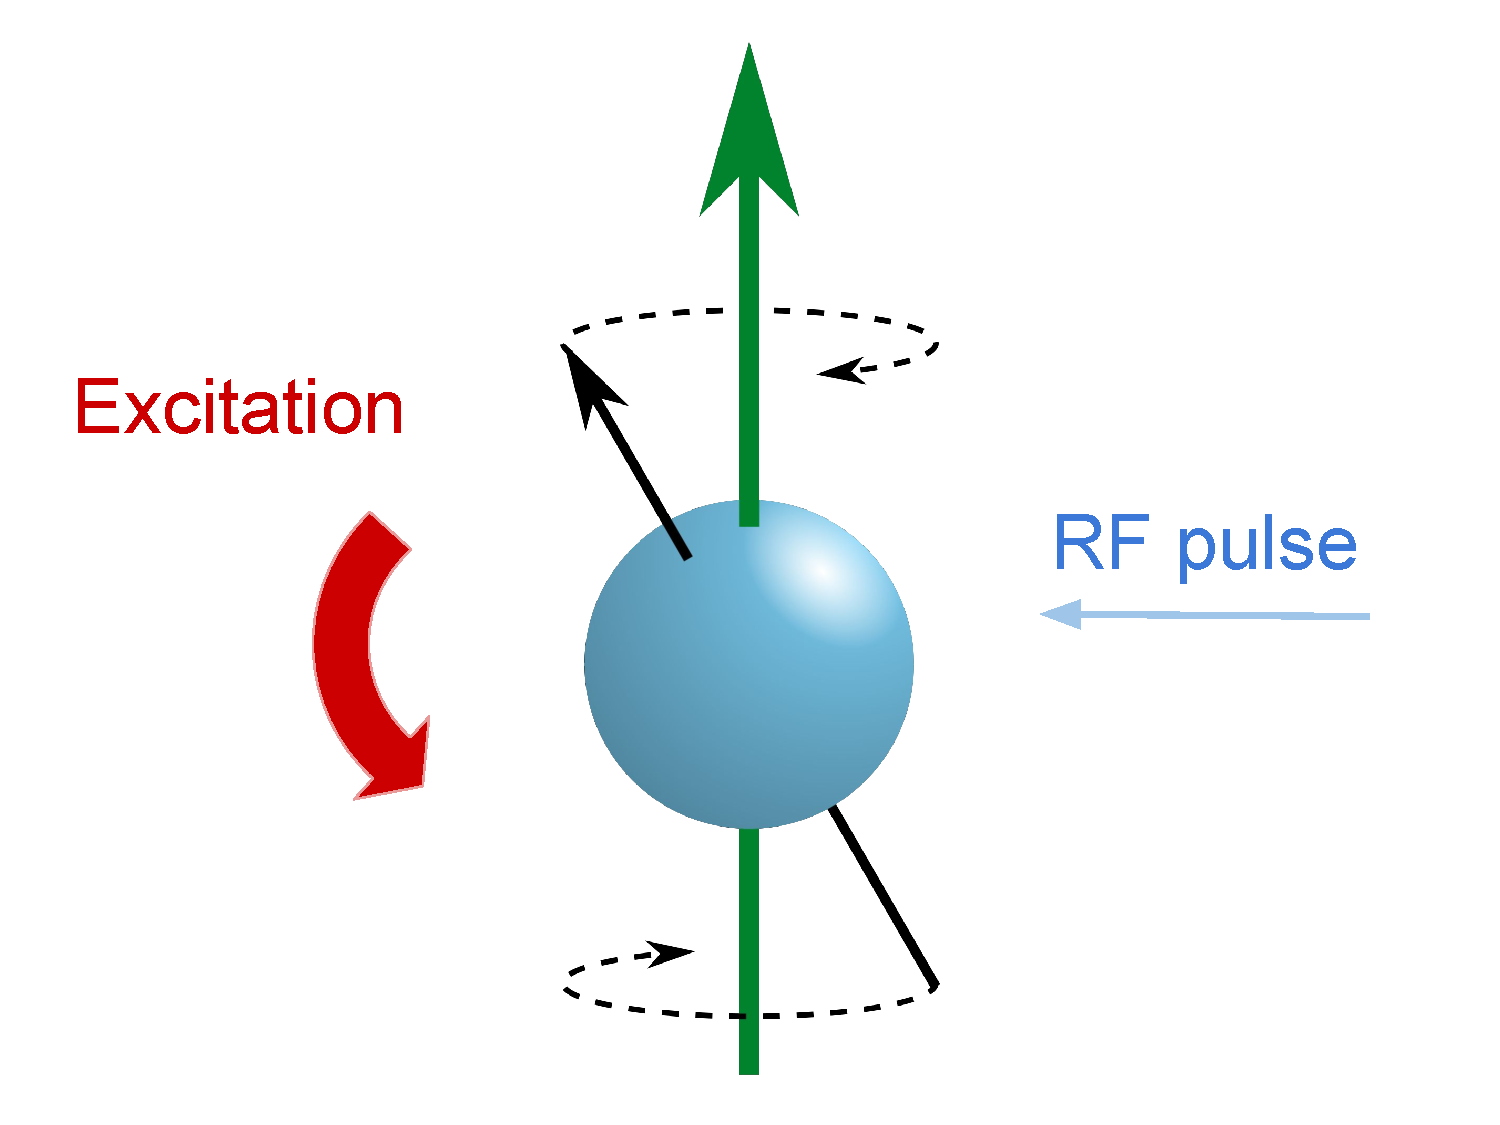
\includegraphics[width=0.5\textwidth]{Figures/intro_figures/Excitation.pdf}
        \caption{\label{fig:excitation}\textbf{Illustration of the excitation phenomenon:} the blue arrow represents an incoming RF~(Radio Frequency) pulse. Illustration courtesy of \citet{wiki}.}
    \end{figure}
    }
    \only<3>{
    \begin{figure}
        \centering
        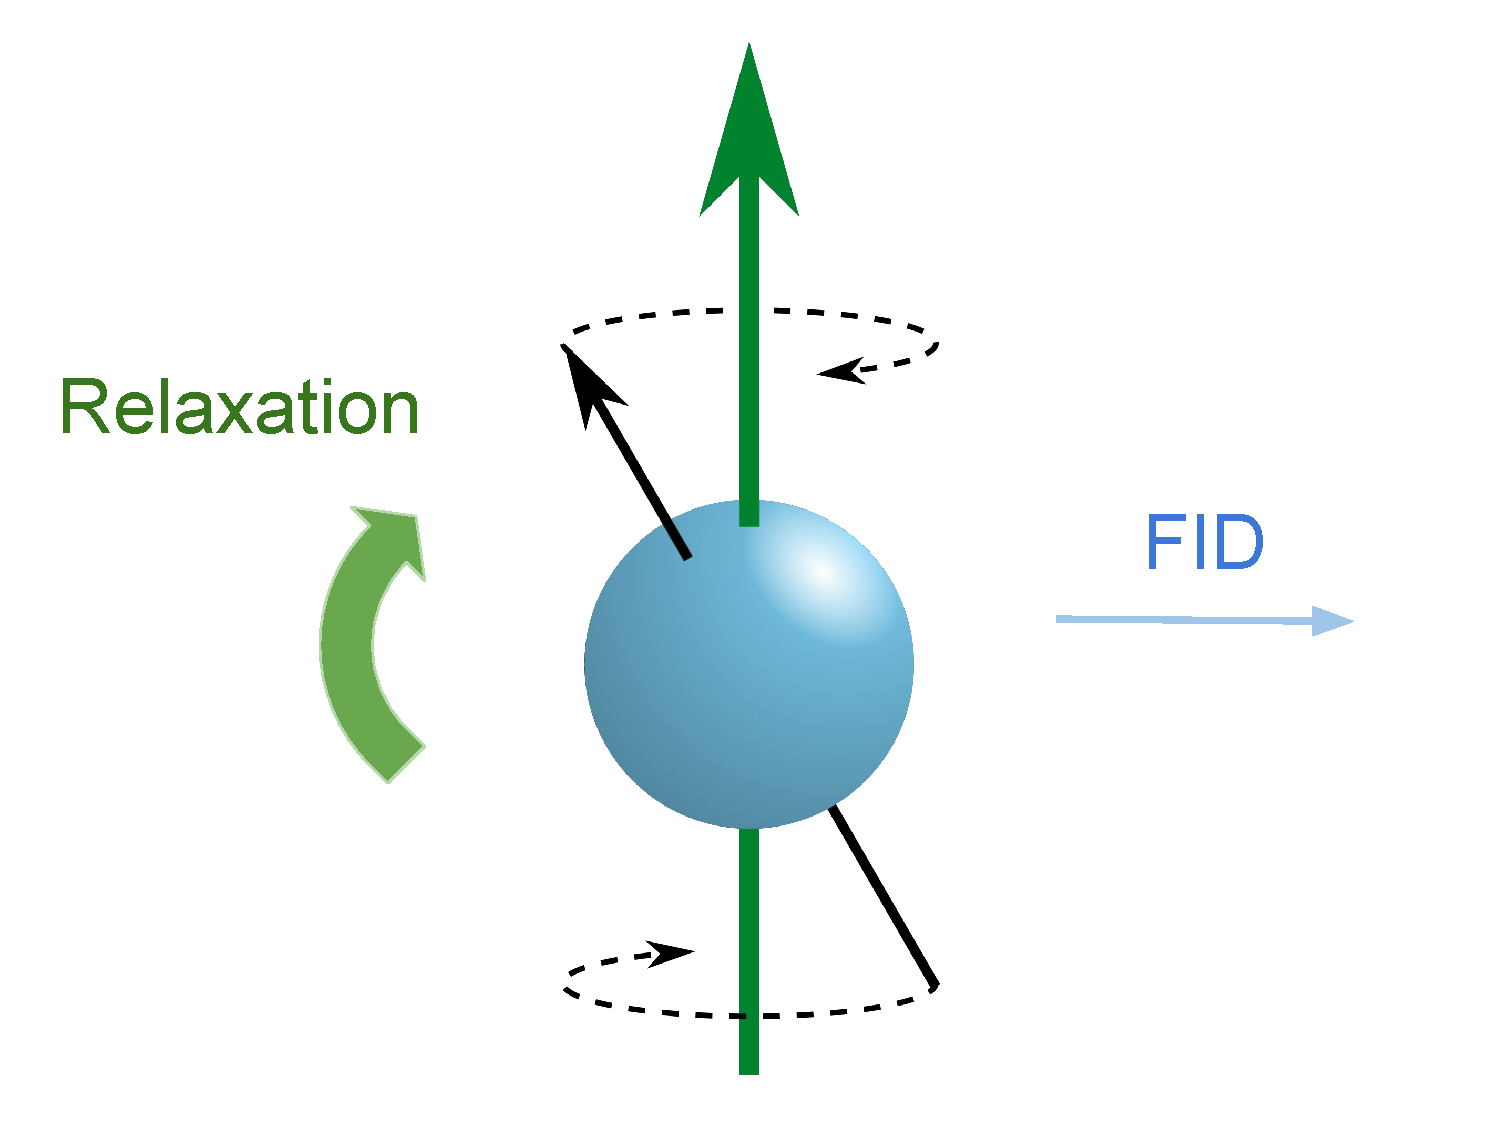
\includegraphics[width=0.5\textwidth]{Figures/intro_figures/Relaxation.pdf}
        \caption{\label{fig:relaxation}\textbf{Illustration of the relaxation phenomenon:} the blue arrow represents an outgoing FID~(Free Induction Decay) pulse. Illustration courtesy of \citet{wiki}.}
    \end{figure}
    }
    % video of e-MRI
\end{frame}

\begin{frame}{Physics of MRI - 2}
    % Because all spins get excited, we get a global RF pulse that is the weighted sum of the contribution of all spins' relaxation RF pulses: global information
    % We can obtain "multiple global information", by changing a bit the magnetic field spatially using gradients
    % Signal equation
    However, the FID carries global information.
    \pause
    
    Using magnetic gradients enables changing a bit the magnetic field spatially, and therefore changing the global information depending on local factors.
    \pause
    
    This allows us to receive a temporal signal of the form:
    \begin{equation*}
        \vspace{\baselineskip}
        \tikzmarknode{S}{\highlight{blue}{$S_{tr}(t)$}} \propto \omega_0  \int_{V_s} B_{tr} \tikzmarknode{M}{\highlight{green}{$M_{tr}(t, \rb)$}} e^{-\imath \gamma \rb \cdot \int_0^t \tikzmarknode{G}{\highlight{red}{$\Gb(\tau)$}}  \dif \tau} \dif \rb 
    \end{equation*}
    \begin{tikzpicture}[overlay,remember picture,>=stealth,nodes={align=left,inner ysep=1pt},<-]
        % For "S"
        \onslide<4->{
        \path (S.south) ++ (0,-2em) node[anchor=south east,color=blue!67] (exp_S){\textbf{Recorded MR signal}};
        \draw [color=blue!87](S.south) |- ([xshift=-0.3ex,color=blue]exp_S.south west);
        }
        % For "M"
        \onslide<5->{
        \path (M.south) ++ (0, -6em) node[anchor=south east,color=green!47] (exp_M){\textbf{Magnetic field in each location $\rb$,}\\ \textbf{proportional to the spin density $\rhob(\rb)$}};
        \draw [color=green!87](M.south) |- ([xshift=-0.3ex,color=green]exp_M.south west);
        }
        % For "G"
        \onslide<6->{
        \path (G.south) ++ (0, -2em) node[anchor=north west,color=red!47] (exp_G){\textbf{Temporal gradients,}\\\textbf{controlled by the operator}};
        \draw [color=red!87](G.south) |- ([xshift=-0.3ex,color=red]exp_G.south east);
        }
    \end{tikzpicture}
\end{frame}

\begin{frame}{Physics of MRI - 3}
    % Signal equation => k-space
    The k-space vector, $\kb(t) = \frac{\gamma}{2\pi} \int_0^t \Gb(\tau) \dif \tau$, defines how we traverse the Fourier space of the anatomical image.

    % We are sampling in the Fourier space of the anatomical image
    \begin{figure}
        \centering
        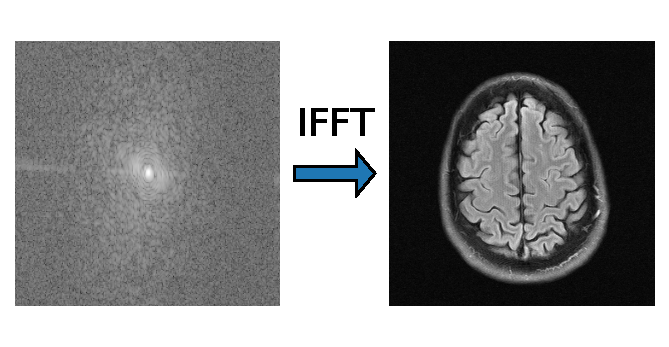
\includegraphics[height=0.4\textheight]{Figures/intro_figures/kspace_to_image.pdf}
        \caption{\label{fig:example-kspace}\textbf{Example of a k-space with its corresponding anatomical image}: The raw data is from the fastMRI dataset. The k-space is in log-scale and only the magnitude of the 2 images are represented. We selected only a single coil from the 16 coils available for illustrative purposes.}
    \end{figure}
\end{frame}

\begin{frame}{Physics of MRI - 4}
    % Let's not forget our initial goal here: we want to understand why MRI is slow
    % The relaxation is slow !
    \begin{block}{Recap}
        MRI relies on the nuclear resonance phenomenon. This enables us to sample the Fourier space of the anatomical object of interest.
    \end{block}
    \pause
    MRI is slow, because the relaxation is slow!
\end{frame}

\subsection{Acceleration in MRI}
\begin{frame}{Where is there room for acceleration?}
    % Explain the concept of redundancy
    % first example: partial Fourier => give limits
    \textbf{Redundancy}, otherwise called \textbf{sparsity, symmetry, structure or a priori information}, is the core concept that will help us accelerate MRI.\\
    
    \begin{overprint}
        \onslide<2>
        \hfill \break
    Here is an illustrative example:
    \begin{figure}
        \centering
        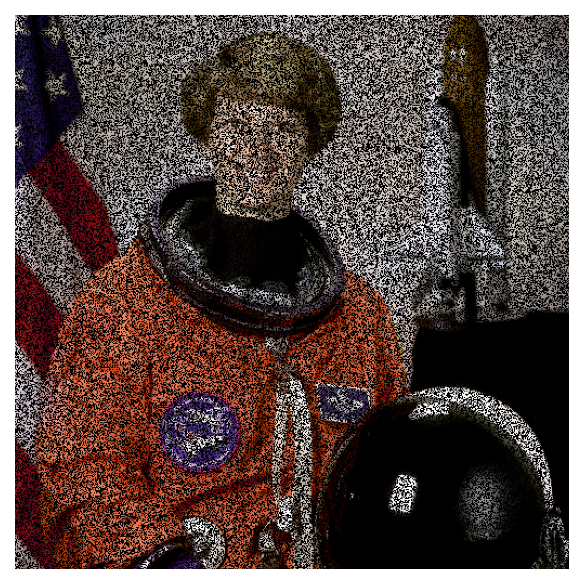
\includegraphics[height=0.4\textheight]{Figures/intro_figures/astronaut_masked.pdf}
        \caption{\label{fig:astronaut-masked}\textbf{The inpainting problem.} Even without access to all the pixel values directly, we can infer them, because the information in the image is redundant.
        }
    \end{figure}
    
    \onslide<3>
    \hfill \break
    Here is an illustrative example:
    \begin{figure}
        \centering
        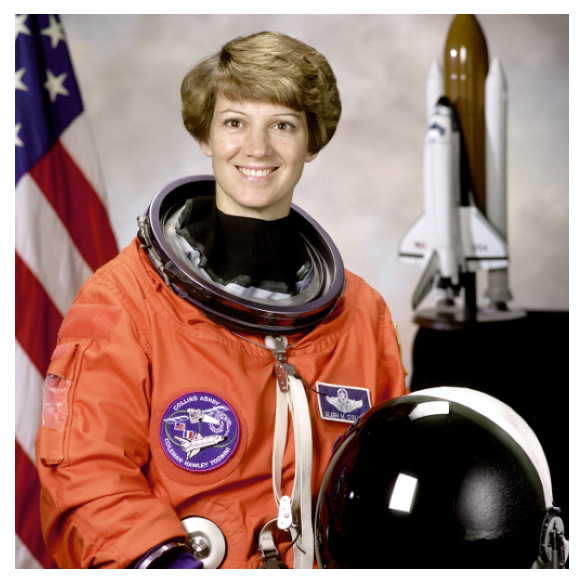
\includegraphics[height=0.4\textheight]{Figures/intro_figures/astronaut.pdf}
        \caption{\label{fig:astronaut}\textbf{The inpainting problem.} Even without access to all the pixel values directly, we can infer them, because the information in the image is redundant.
        }
    \end{figure}
    
    \onslide<4>
        \hfill \break
        Is there a similar thing in MRI?

        Yes! The anatomical image is real-valued so its Fourier Transform~(FT) has a conjugate symmetry.
        Using this redundancy to sample less points in the k-space (i.e. using the relaxation fewer times) is a technique called \textbf{Partial Fourier}.
        
        But in practice it is still needed to sample 6/8 of the Fourier space (acceleration of 1.3).\footfullcite{emri}
    
    \end{overprint}
    
\end{frame}

\begin{frame}{Parallel imaging}
    % "forging" the redundancy
    We can build more redundancy in the measuring system by using \textbf{more antennas (called coils)} to measure the magnetic signal.
    
    This technique is called \textbf{Parallel Imaging~(PI)}. 
    A reconstruction algorithm is now needed to handle the multi-coil undersampled data.
        \textbf{SENSE}\footfullcite{Pruessmann1999SENSE:MRI} and \textbf{GRAPPA}\footfullcite{Griswold2002GeneralizedGRAPPA} are such algorithms.    
    % GRAPPA + SENSE examples
\end{frame}

\begin{frame}{The example of GRAPPA}
    \begin{figure}
        \centering
        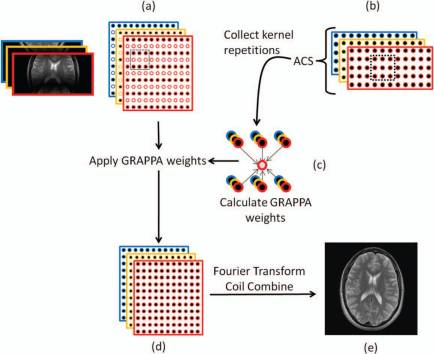
\includegraphics[height=0.6\textheight]{Figures/intro_figures/GRAPPA.jpeg}
        \caption{\label{fig:GRAPPA}\textbf{GRAPPA illustration.} Image courtesy of \citet{deshmane2012parallel}.
        }
    \end{figure} 
\end{frame}

\begin{frame}{Limits of Parallel Imaging}
    % Max AF
    % XXX: wait for AV's response
    % ow: https://www.siemens-healthineers.com/magnetic-resonance-imaging/options-and-upgrades/clinical-applications/syngo-grappa says 2,3
\end{frame}

\section{Compressed Sensing}
\begin{frame}{Another look at redundancy: the prior point of view}
    % give a sense of what structure is and how it relates to redundancy
    Redundancy is not always strict: we may only have a strong correlation between 2 structures of the image.
    \begin{figure}
        \centering
        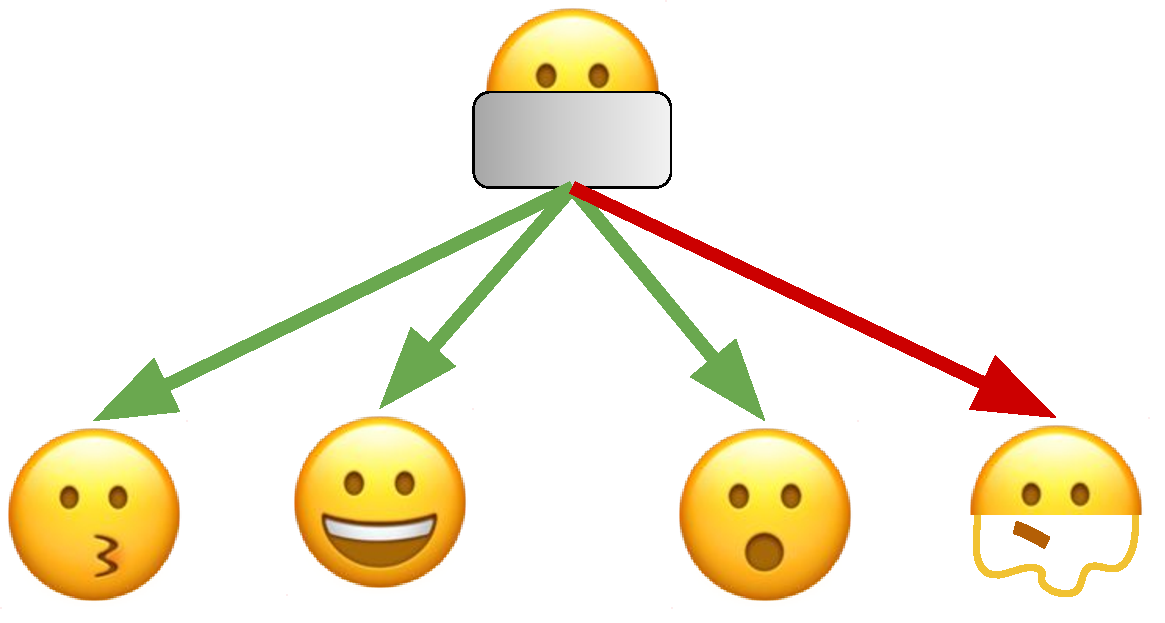
\includegraphics[height=0.5\textheight]{Figures/cs_figures/smiley_prior.pdf}
        \caption{\label{fig:redundancy-smiley}\textbf{A smiley example to a priori knowledge:} Even if we do not have access to the whole image, we still know which images are more \emph{likely} to correspond to it.
        }
    \end{figure}
\end{frame}

\subsection{Linear Inverse Problems}
\begin{frame}{Linear Inverse Problems}
    % introduce linear inverse problems
    To leverage this type of redundancy, we introduce the concept of \textbf{Linear Inverse Problems}:
    \begin{equation*}
        \tikzmarknode{A}{\highlight{green}{$\Ab$}} \tikzmarknode{x}{\highlight{blue}{$\xb$}} = \tikzmarknode{y}{\highlight{yellow}{$\yb$}}
    \end{equation*}
    \vspace{2.5\baselineskip}
    \begin{tikzpicture}[overlay,remember picture,>=stealth,nodes={align=left,inner ysep=1pt},<-]
        % For "A"
        \onslide<6>{
        \path (A.south) ++ (0,-2em) node[anchor=south east,color=green!47] (exp_A){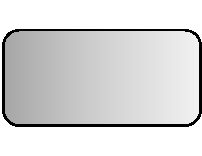
\includegraphics[width=0.05\textwidth]{Figures/intro_figures/smiley_prior_forw_op.pdf}};
        \draw [color=green!87](A.south) |- ([xshift=-0.3ex,color=green]exp_A.south west);
        }
        \onslide<7->{
        \path (A.south) ++ (0,-2em) node[anchor=south east,color=green!47] (exp_A){\textbf{Measurement operator}};
        \draw [color=green!87](A.south) |- ([xshift=-0.3ex,color=green]exp_A.south west);
        }
        % For "x"
        \onslide<2>{
            \path (x.south) ++ (0, -4.5em) node[anchor=south east,color=blue!67] (exp_x){
\includegraphics[width=0.05\textwidth]{Figures/intro_figures/smiley_prior_x.pdf}};
        \draw [color=blue!87](x.south) |- ([xshift=-0.3ex,color=blue]exp_x.south west);
        }
        \onslide<3->{
        \path (x.south) ++ (0, -4.5em) node[anchor=south east,color=blue!67] (exp_x){\textbf{Signal to reconstruct}};
        \draw [color=blue!87](x.south) |- ([xshift=-0.3ex,color=blue]exp_x.south west);
        }
        % For "y"
        \onslide<4>{
            \path (y.south) ++ (0, -1em) node[anchor=north west,color=yellow!67] (exp_y){
\includegraphics[width=0.05\textwidth]{Figures/intro_figures/smiley_prior_y.pdf}};
            \draw [color=yellow!87](y.south) |- ([xshift=-0.3ex,color=yellow]exp_y.south east);
        }
        \onslide<5->{
        \path (y.south) ++ (0, -1em) node[anchor=north west,color=yellow!67] (exp_y){\textbf{Measurements}};
        \draw [color=yellow!87](y.south) |- ([xshift=-0.3ex,color=yellow]exp_y.south east);
        }
    \end{tikzpicture}
    

    \onslide<8->{
    Problems arise when $\ker{\Ab} \neq \{0\}$, i.e. when there are multiple solutions to this equation.
    }

    \onslide<9->{
    \hfill \break
    In order to select one of these solutions, we need to use a priori knowledge.
    }
\end{frame}

\begin{frame}{Sparsity and Inverse Problems}
    % explain the concept of sparsity and its link to recovery guarantees
    \begin{definition}[Sparsity]
        A vector $\xb \in \mathbb{C}^n$ is called $s$-sparse if it contains at most $s$ non-zero entries.
    \end{definition}

    \begin{lemma}[Optimization reformulation of sparse vector recovery~\citep{Foucart2013SparseSystems}]
        For a given sparsity $s$, and $s$-sparse vector $\xb$:
    \begin{enumerate}[(a)]
        \item The vector $\xb$ is the unique $s$-sparse solution of $\Ab \xb = \yb$, that is $\{\zb \in \mathbb{C}^n : \Ab \zb = \Ab \xb, \|z\|_0 \leq s\} = \{\xb\}$
        \item The vector $\xb$ can be reconstructed as the unique solution of:
        \begin{equation*}
            \label{eq:cs-problem-l0-min}
            \min_{\zb \in \mathbb{C}^n} \|\zb\|_0 \quad \text{subject to} \quad \Ab \zb = \yb
        \end{equation*}
    \end{enumerate}
    \end{lemma}
\end{frame}

\begin{frame}{Recovery guarantees}
    \begin{theorem}[{{\citep[Theorem~2.13]{Foucart2013SparseSystems}}}]
        The following properties are equivalent:
\begin{enumerate}[(a)]
    \item Every $s$-sparse vector $\xb \in \mathbb{C}^n$ is the unique $s$-sparse solution of $\Ab \zb = \Ab \xb$, that is, if $\Ab \xb = \Ab \zb$ and both $\xb$ and $\zb$ are $s$-sparse, then $\xb = \zb$.
    \item The null space $\ker(\Ab)$ does not contain any $2s$-sparse vector other than the zero.
    \item Every set of $2s$ columns of $\Ab$ is linearly independent.
\end{enumerate}
    \end{theorem}
\end{frame}

\begin{frame}{Application to MRI}
    MR images themselves cannot be represented as sparse vectors directly, we need a way to express them as such.
    \citet{Lustig2007} did that by using the fact that MR images can be represented sparsely in a \textbf{wavelet} basis.

    \hfill \break
    The Inverse Problem becomes:
    \begin{equation*}
        \tikzmarknode{FS}{\highlight{green}{$\left(\Ib_L\otimes {\mathcal{F}}_{\Omega}\right)\Sbb$}} \tikzmarknode{x}{\highlight{blue}{$\xb$}} = \tikzmarknode{y}{\highlight{yellow}{$\ybb$}}
    \end{equation*}
    \begin{tikzpicture}[overlay,remember picture,>=stealth,nodes={align=left,inner ysep=1pt},<-]
        % For "FS"
        \onslide<4>{
        \path (FS.south) ++ (0,-4em) node[anchor=south east,color=green!47] (exp_FS){
            \textbf{$\mathcal{F}_{\Omega}$ : FT on the $\Omega$ set;}\\
            \textbf{$\Sbb=[\Sb_1^H,\ldots, \Sb_L^H]^\top$: the sensitivity maps}\\
            \textbf{per coil}
        };
        \draw [color=green!87](FS.south) |- ([xshift=-0.3ex,color=green]exp_FS.south west);
        }
        \onslide<5>{
        \path (FS.south) ++ (0,-4em) node[anchor=south east,color=green!47] (exp_FS){
            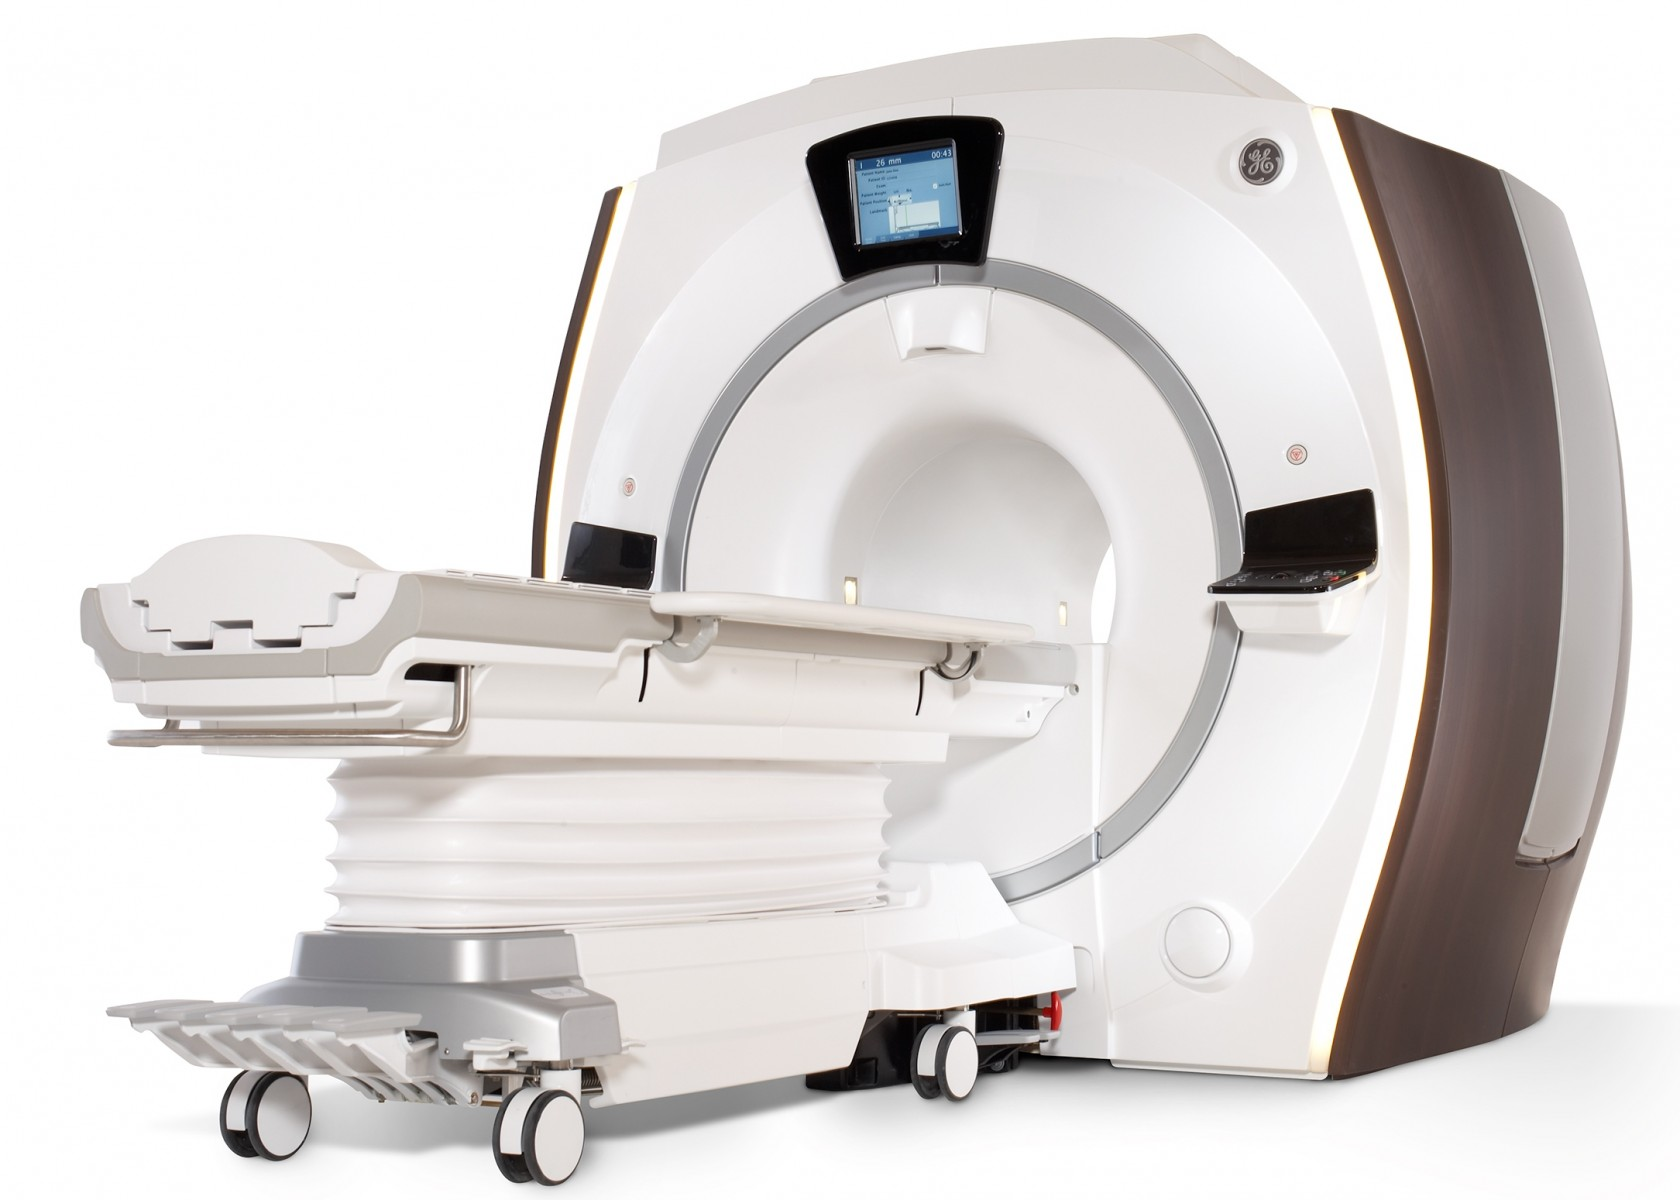
\includegraphics[width=0.1\textwidth]{Figures/intro_figures/mri.jpg}
        };
        \draw [color=green!87](FS.south) |- ([xshift=-0.3ex,color=green]exp_FS.south west);
        }
        % For "x"
        \onslide<2-4>{
        \path (x.south) ++ (0, -2em) node[anchor=south west,color=blue!67] (exp_x){\textbf{2D or 3D MR image}};
        \draw [color=blue!87](x.south) |- ([xshift=-0.3ex,color=blue]exp_x.south east);
        }
        \onslide<5->{
        \path (x.south) ++ (0, -4em) node[anchor=south west,color=blue!67] (exp_x){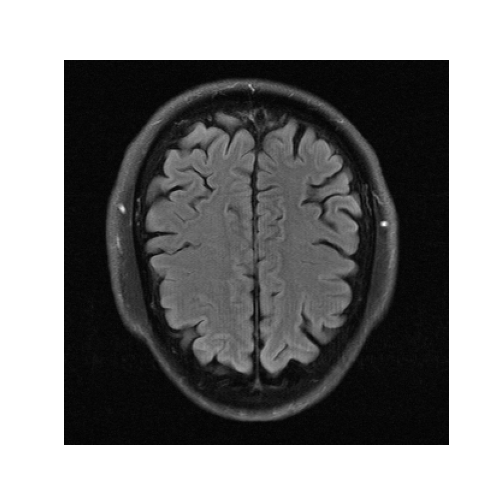
\includegraphics[width=0.1\textwidth]{Figures/intro_figures/brain_mri.png}};
        \draw [color=blue!87](x.south) |- ([xshift=-0.3ex,color=blue]exp_x.south east);
        }
        % For "y"
        \onslide<3-4>{
        \path (y.north) ++ (0, 1em) node[anchor=south west,color=yellow!67] (exp_y){$\ybb=[\yb_1^H, \ldots, \yb_L^H]^\top$,\\ \textbf{k-space measurements} \\ \textbf{for each coil}};
        \draw [color=yellow!87](y.north) |- ([xshift=-0.3ex,color=yellow]exp_y.south east);
        }
        \onslide<5->{
        \path (y.north) ++ (0, 1em) node[anchor=south west,color=yellow!67] (exp_y){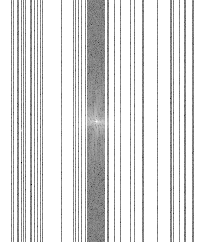
\includegraphics[width=0.07\textwidth]{Figures/intro_figures/kspace_mri.png}};
        \draw [color=yellow!87](y.north) |- ([xshift=-0.3ex,color=yellow]exp_y.south east);
        }
    \end{tikzpicture}
\end{frame}

\subsection{Recovery Algorithms}
\begin{frame}{Relaxation}
    Now we have an optimization problem to solve, but can we?
    \pause
    No; we need to relax it using the basis pursuit:
    \begin{equation*}
        \label{eq:basis-pursuit}
        \min_{\xb \in \mathbb{C}^n} \|\xb\|_1 \quad \text{subject to} \quad \Ab \xb = \yb
    \end{equation*}

    \pause
    For this problem to have the same solutions as the non-relaxed one, we need coherence-based constraints on the measurement operator $\Ab$.

\end{frame}

\begin{frame}{The canonical MRI reconstruction problem}
    We introduce the notion of a sparsity basis $\psib$ and the fact that the measurements can be noisy to obtain the canonical MRI reconstruction problem:
    \begin{equation*}
        \min_{\xb \in \mathbb{C}^n} \overbrace{\|\tikzmarknode{calA}{\underline{\mathcal{A}}} \xb - \yb \|_2^2}^{\text{\sf \footnotesize Data consistency}}  + \overbrace{ \tikzmarknode{lambda}{\underline{\lambda}} \|\psib \xb\|_1}^{\text{\sf \footnotesize Regularization term } }
    \end{equation*}
    \vspace{\baselineskip}
    \begin{tikzpicture}[overlay,remember picture,>=stealth,nodes={align=left,inner ysep=1pt},<-]
        % For "calA"
        \path (calA.south) ++ (0,-2.5em) node[anchor=south east,color=black!87] (exp_calA){
            $= \left(\Ib_L\otimes {\mathcal{F}}_{\Omega}\right)\Sbb$
        };
        \draw [color=black!87](calA.south) |- ([xshift=-0.3ex,color=black]exp_calA.south west);
        % For "lambda"
        \path (lambda.south) ++ (0, -2.5em) node[anchor=south west,color=black!87] (exp_lambda){
            Regularization hyperparameter
        };
        \draw [color=black!87](lambda.south) |- ([xshift=-0.3ex,color=black]exp_lambda.south east);
    \end{tikzpicture}
    
\end{frame}

\begin{frame}{ISTA}
     The Iterative Shrinkage-Thresholding Algorithm~(ISTA) can be used to solve the canonical MRI reconstruction problem:
     \begin{equation*}
        \label{eq:ista-step}
        \begin{split}
            \xb_{n+1} &= \xb_n - \epsilon_n \mathcal{A}^H\left(\mathcal{A} \xb_n - \ybb\right)\\
            \xb_{n+1} &= \tikzmarknode{prox}{\operatorname{prox}}_{\epsilon_n \tikzmarknode{reg}{\mathcal{R}}}\left(\xb_{n+1}\right)
        \end{split}
    \end{equation*}
    \begin{tikzpicture}[overlay,remember picture,>=stealth,nodes={align=left,inner ysep=1pt},<-]
        % For "prox"
        \path (prox.south) ++ (0,-2.5em) node[anchor=south east,color=black!87] (exp_prox){
            Proximity operator
        };
        \draw [color=black!87](prox.south) |- ([xshift=-0.3ex,color=black]exp_prox.south west);
        % For "reg
        \path (reg.south) ++ (0, -2.5em) node[anchor=south west,color=black!87] (exp_reg){
            \footnotesize $= \|\psib \cdot\|_1$
        };
        \draw [color=black!87](reg.south) |- ([xshift=-0.3ex,color=black]exp_reg.south east);
    \end{tikzpicture}
\end{frame}

% \begin{frame}{Dictionary Learning}

% \end{frame}


\begin{frame}{Limitations of classical recovery algorithms}
    % give max AF
    % also give a sense of the limitations in compute and in prior learning
    Additional acceleration factor on top of PI: 1.5. % from https://www.philips.fr/healthcare/ressources/landing/the-next-mr-wave/compressed-sense
    \pause
    The prior knowledge expressed by the wavelet basis (or other basis) is limited: handcrafted and linear.
\end{frame}

\begin{frame}{Compressed Sensing}
    \begin{block}{Recap}
        MRI is slow because of relaxation. 
        
        We can use redundancy in many forms to reduce the amount of samples we need in the Fourier space, and therefore the number of relaxations.
        
        But we are limited by simple forms of redundancy.
    \end{block}
\end{frame}

\section{Deep Learning}

\subsection{The power of Deep Learning}
\begin{frame}{The power of Deep Learning}
    % we want to learn a complicated function that tells us whether an image is an MR image
    % similarly deep learning has been able to build functions that tell whether an image is that of a dog or a cat
    % universal approx
    We want to learn a complicated function that tells us whether a complex-valued vector is an MR image or not.
    \pause

    Deep Learning~(DL) has been used to build such functions:
    % XXX: image that does f_theta(Dog Image) -> dog
\end{frame}

\begin{frame}{Formalism - 1}
    % supervised learning objective function
    The classical framework for DL is supervised learning:
    \vspace{\baselineskip}

    \begin{equation*}
        \argmin_{\tikzmarknode{params}{\highlight{orange}{$\thetab \in \Theta$}}} \tikzmarknode{sum}{\highlight{purple}{$\sum\limits_{(\xb_i, \yb_i) \in \mathcal{D}}$}} \tikzmarknode{loss}{\highlight{green}{$\mathcal{L}$}}(\tikzmarknode{nn}{\highlight{brown}{$f_{\thetab}$}} (\tikzmarknode{input}{\highlight{blue}{$\xb_i$}}), \tikzmarknode{label}{\highlight{red}{$\yb_i$}}, \thetab)
    \end{equation*}
    \begin{tikzpicture}[overlay,remember picture,>=stealth,nodes={align=left,inner ysep=1pt},<-]
        % For "input"
        \onslide<2->{
        \path (input.north) ++ (0,1.5em) node[anchor=south west,color=blue!87] (exp_input){
            input};
        \draw [color=blue!87](input.north) |- ([xshift=-0.3ex,color=blue]exp_input.south east);
        }
        % For "label"
        \onslide<3->{
        \path (label.south) ++ (0, -2.5em) node[anchor=south west,color=red!87] (exp_label){
            label};
        \draw [color=red!87](label.south) |- ([xshift=-0.3ex,color=red]exp_label.south east);
        }
        % For "nn"
        \onslide<4->{
        \path (nn.south) ++ (0, -4.5em) node[anchor=south east,color=brown!87] (exp_nn){
            neural network};
        \draw [color=brown!87](nn.south) |- ([xshift=-0.3ex,color=brown]exp_nn.south west);
        }
        % For "loss"
        \onslide<5->{
        \path (loss.north) ++ (0, 1.5em) node[anchor=south west,color=green!47] (exp_loss){
            loss};
        \draw [color=green!47](loss.north) |- ([xshift=-0.3ex,color=green]exp_loss.south east);
        }
        % For "sum"
        \onslide<6->{
        \path (sum.south) ++ (0, -2em) node[anchor=south east,color=purple!87] (exp_sum){
            Estimator of the expected value};
        \draw [color=purple!87](sum.south) |- ([xshift=-0.3ex,color=purple]exp_sum.south west);
        }
        
        % For "params"
        \onslide<7->{
        \path (params.west) ++ (-2em, 0) node[anchor=east,color=orange!87] (exp_params){
            Parameters};
        \draw [color=orange!87](params.west) -- ([xshift=-0.3ex,color=orange]exp_params.east) -- ([xshift=-0.3ex,color=orange]exp_params.south east) -- ([xshift=-0.3ex,color=orange]exp_params.south west);
        }
        
    \end{tikzpicture}
\end{frame}

\begin{frame}{Formalism - 2}
    % Stochastic Gradient descent and chain rule
\end{frame}

\subsection{Requirements for Deep Learning}
\begin{frame}{Requirements for Deep Learning}
    % Great that I can do that, but does it take ?
    % Data, compute + memory, framework
    % accept that it's "black-box"
\end{frame}

\begin{frame}{Building the network}
    % give classical functions
\end{frame}

\addtocontents{toc}{\newpage}

\section{Deep Learning for MRI}
\subsection{Simple models}
\begin{frame}{Model agnostic learning}
    % reframing the problem as supervised learning
    % no knowledge of the physics imposed in the model
\end{frame}

\begin{frame}{Single domain learning}
    % Use the backward operator as a basis for the restoration model
\end{frame}

\subsection{Unrolled models}
\begin{frame}{Unrolled models - 1}
    % recovery algorithm and corresponding computation graph
    % show on second slice unrolled computation graph
\end{frame}

\begin{frame}{Unrolled models - 2}
    % move from fixed prior to learned one
\end{frame}

\begin{frame}{Unrolled models - 3}
    % first benchmark: different unrolling strategies give different results

\end{frame}

\subsection{New unrolled models}
\begin{frame}{XPDNet}
    % talk about XPDNet archi
\end{frame}

\begin{frame}{fastMRI challenge}
    % mention fastMRI challenge results
\end{frame}

\begin{frame}{NC-PDNet - 1}
    % explain NC-PDNet and density compensation
\end{frame}

\begin{frame}{NC-PDNet - 2}
    % give results
\end{frame}

\begin{frame}{Recap}
    % cool: we are starting to have good results, let's not forget the end goal
    % use this in a scanner so that the MRI exam is faster
    % how will this technique fare in the clinical setting ?
\end{frame}

\section{Clinical applicability}
\subsection{Learnlets}
\begin{frame}{Learnlets - 1}
    % explain that robustness is a key aspect that we have with wavelets
\end{frame}

\begin{frame}{Learnlets - 2}
    % show the Learnlets model
\end{frame}

\begin{frame}{Learnlets - 3}
    % Learnlets results
\end{frame}

\subsection{Denoising Score Matching}
\begin{frame}{Denoising Score Matching - 1}
    % explain what UQ might be used for
\end{frame}

\begin{frame}{Denoising Score Matching - 2}
    % give method of DSM
\end{frame}

\begin{frame}{Denoising Score Matching - 3}
    % give results
\end{frame}

\subsection{Comparison with GRAPPA}
\begin{frame}{Prospective comparison with GRAPPA}
    % show big brain results
    % explain why it's robustness test already
\end{frame}

\begin{frame}{Recap}
    % we have seen how to adapt to clinical setting and answered the question of prospective reconstruction
    % robust : learnlets
    % UQ: DSM
    % propsective: check
\end{frame}

\section{Going even deeper}
\subsection{Implicit models}

\begin{frame}{Why should we go deeper?}
    % with deeper models, comes better performance
    % figure of Pezzotti et al.
\end{frame}

\begin{frame}{Can we go deeper?}
    % in the current state not: activations + constrained memory
\end{frame}

\begin{frame}{The modeling solutions}
    % gradient checkpointing
    % Invertible networks
    % Implicit models
\end{frame}

\begin{frame}{Deep Equilibrium networks}
    % give equation and how to compute the gradient with IFT
\end{frame}

\subsection{SHINE}
\begin{frame}{The limits of DEQs}
    % they are slow to train
\end{frame}

\begin{frame}{Why are DEQs slow?}
    % bc of Jacobian inversion
\end{frame}

\begin{frame}{Can we avoid the Jacobian inversion?}
    % yes: reuse a by-product of the forward pass, share the inverse estimate
\end{frame}

\begin{frame}{Application to Hyperparameter optimization}
    % it's also a bilevel prob
\end{frame}

\begin{frame}{Results on DEQs}

\end{frame}

\section{Conclusion \& Future works}

\begin{frame}{Conclusion}
    % what have we seen so far in the journey?
\end{frame}

\begin{frame}{Future works}
    % DEQs for MRI recon
    % More operator correction
    % Trajectory learning
\end{frame}
%----------------------------------------------------------------------------------------

\begin{frame}[allowframebreaks]{References}
    \printbibliography
\end{frame}

\end{document}